% 请确保文件编码为utf-8,使用XeLaTex进行编译,或者通过overleaf进行编译

\documentclass[answers]{exam}  % 使用此行带有作答模块
% \documentclass{exam} % 使用此行只显示题目

\usepackage{xeCJK}
\usepackage{zhnumber}
\usepackage{graphicx}
\usepackage{hyperref}
\usepackage{amsmath}
\usepackage{amssymb}
\usepackage{mathtools}
\usepackage{booktabs}
\usepackage{enumerate}
\usepackage{enumitem} % 控制列表样式
\usepackage{listings} 

\title{2025自然语言处理 \\ 课程设计1}
\date{2025.4.1}
\pagestyle{headandfoot}
\author{人工智能学院 221300079 王俊童}
\firstpageheadrule
\firstpageheader{南京大学}{2025自然语言处理}{课程设计1}
\runningheader{南京大学}
{2025自然语言处理}
{课程设计1}
\runningheadrule
\firstpagefooter{}{第\thepage\ 页(共\numpages 页)}{}
\runningfooter{}{第\thepage\ 页(共\numpages 页)}{}

% no box for solutions
% \unframedsolutions
\def \x \mathbf{x}


\setlength\linefillheight{.5in}

% \renewcommand{\solutiontitle}{\noindent\textbf{答:}}
\renewcommand{\solutiontitle}{\noindent\textbf{解:}\par\noindent}

\renewcommand{\thequestion}{\zhnum{question}}
\renewcommand{\questionlabel}{\thequestion .}
\renewcommand{\thepartno}{\arabic{partno}}
\renewcommand{\partlabel}{\thepartno .}

% 实验报告需包含以下内容:

% 实现了哪些方法并对自己设计的代码模块用简洁的语言描述
% 如何复现主要实现结果,包括执行命令和环境依赖,
% 建议修改requirement.txt和新建bash文件来展示如何运行代码
% 不同方法的实验结果如何
% 遇到的具体问题,如何解决
% 对该任务和在探索过程中的思考


\begin{document}
% \normalsize
\maketitle
综述,首先观察代码结构,逻辑如下:
\begin{itemize}
    \item 命令行参数解析。有method,是否analyze,statistical里面方法的选取。
    \item 加载数据和数据分析(需要我们实现数据分析)
    \item 三个方法的训练:
    \begin{itemize}
        \item rule:基于一些规则得到的一个实现。train有四种纠错规则:
        \begin{itemize}
            \item $\_extract\_confusion\_pairs$:字符混淆对提取。
            \item $\_extract\_punctuation\_rules$:标点符号规则提取
            \item $\_extract\_grammar\_rules$:语法规则提取
            \item $\_extract\_word\_confusion$:词汇混淆对提取
        \end{itemize}
        然后以上四种错误的纠错发生在correct里面。
        \item statistical:基于统计学习方法的纠错。这个里面又分为两个模型:
        \begin{itemize}
            \item ngram模型:初始化了一堆数据结构,1-4的gram方法,字符混淆矩阵和错误率等
            \item ml模型:用机器学习方法去做。
        \end{itemize}
        \item 集成学习方法,在框架代码的ensemble部分有留给我们实现。
    \end{itemize}
    \item 三个方法对应的纠错和评估。跟上面一样了,可以实现很多的correct方法,都有对应接口。
\end{itemize}
可以看出整个代码框架都还是比较整齐的,我们需要完成的TODO任务如下:
\begin{itemize}
    \item 数据的analyze分析部分和画图。
    \item rule:完成规则方法的实现。完成对应规则方法的纠错改正。
    \item statistical:完成ngram和ml方法的对应修正和改正。
    \item main:完成集成学习方法。
    \item 其余可以加一些深度学习之类的方法实现。
\end{itemize}

\section{实现方法及其简单描述,遇到的问题和解决方案(全包含,就不单独列了,按照我的编程和问题思考思路来写的)}
\subsection{数据分析部分}
数据分析部分,我们将原来的args做了一点点修改,然后我们首先可以根据原词典数据进行统计,把label为1的错误数据中的错误字符全部统计
出来,而且可以得到错误率最高的10个的错误模式和错误字符,这更方便我们后续处理:
\begin{lstlisting}
# 只看错的
if label == 1:  
    error_count += 1
    
    if len(source) == len(target):  
        for i, (s_char, t_char) in enumerate(zip(source, target)):
            if s_char != t_char:
                char_error_freq[s_char] += 1
                error_patterns[(s_char, t_char)] += 1
\end{lstlisting}
然后我们把它可视化, 同时,由于matplotlib不支持中文字体,需要更换自己电脑里面的路径。这个在对应
data analysis的python文件里面有讲。

可以看一个我做出来的效果,还是蛮不错的。
\begin{figure}[h]
    \centering
    \label{error_distribution}
    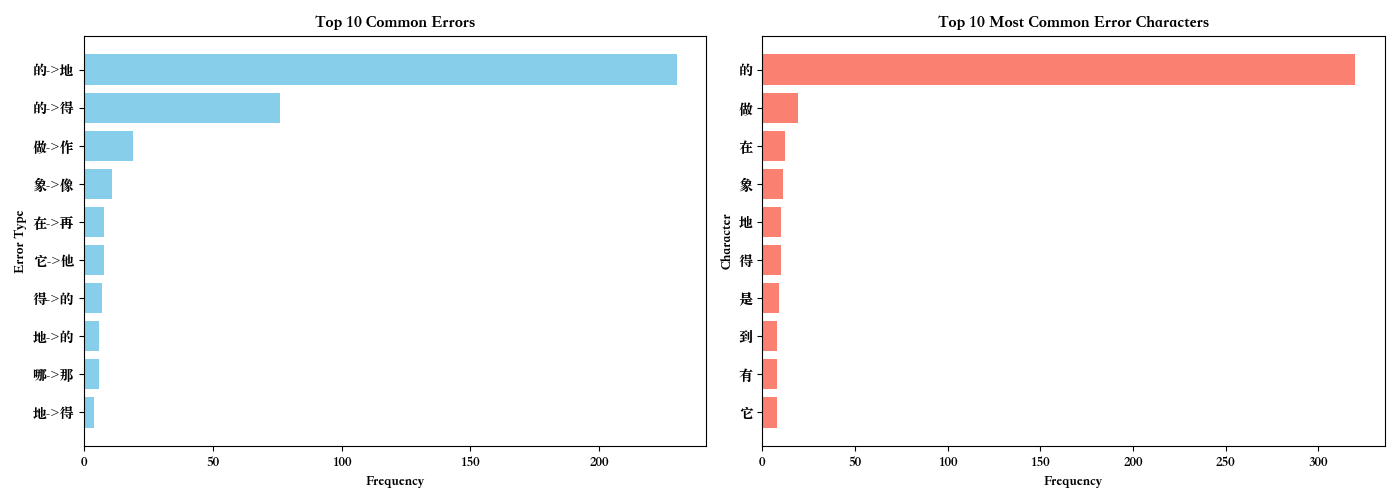
\includegraphics[width=1\textwidth]{../pic/error_distribution.png} 
    \caption{error distribution}  
\end{figure}
可以看到的和地的错误最多,还有的和得之类的,一般都是些同音不同意的字。

\subsection{3个方法部分}
\subsubsection{方法1:rule}
rule这个方法还蛮简单的,基本是基于人类的常识性的方法,有点像是打表。但是肯定有补全不了的规则,这个是硬伤。
共有如下的需要填补的方法:
\begin{itemize}
    \item self.\_extract\_confusion\_pairs:这个方法已经给我们补全了。意思是提取了混淆字符对。
    但是这个一眼就存在一些问题:
    \begin{itemize}
        \item 没有考虑插入和删除的错误
        \item 没有考虑很强烈的上下文特征
        \item 不同的count对于噪声过滤效果不一样,可以产生不一样的效果
    \end{itemize}
    我们首先修改这个混淆对的做法:我们加入一个insert,delete标识,这样就考虑了重复和缺失两个新的情况,然后对于count的噪声
    过滤,我们设一个min\_count,这样就可以随时调控。
    \textbf{但是,我写了之后发现还降低了,真没绷住啊,说明好像不需要考虑这么多,就注释掉了。但是我们保留一个count的修改}
    
    同时我们还尝试让他考虑上下文:$self.confusion\_pairs[s\_char][(t\_char, context)] += 1$,但是好像这样效果更差。
    我们的思考是,引入上下文增加了噪声,反而让这个效果不好了,说明成对出现的错词可能多,而且可能存在故意的行为,我们就干脆不要好了。

    \textbf{BTW,经过我反复尝试,mincount去噪为3效果好,这也证实了我的猜想,上下文反而会增加噪声。}
    \item self.\_extract\_punctuation\_rules : 我的思路是将每一句的标点单独的提取出来,然后对比,看
    哪一个位置的标点不一样,然后就记录。但是事实上好像训练集的标点正确率有点高吧,我只找到了一组有错误的。${'”': defaultdict(<class 'int'>, {',': 1})}$
    那这个就很恶心了,我可能需要自己去补充一些修正规则了。
    \item self.\_extract\_grammar\_rules :我的想法是,可以用一定的词性分析工具来看语法的正确或者错误。我们引入$import jieba.posseg as pseg$。这个库
    可以拿来做词性分析。然后记录每种词性替换 (pos\_replace) 和单词替换 (word\_replace) 出现的次数。我们设置一个置信度,这样就不会乱换一些东西,跟之前的count其实是
    一个东西。我们认为:
    \[confidence = \frac{appear\ counts}{training\ set\ length} \]
    这样就可以避免一些问题。\\
    经过实验,其实我发现这个的作用率很小,因为如果我按照rule直接去设定规则,整个会有能修改的,但是同时也会违背一些规则本身,句法反而
    被改变了,所以高置信度虽然可以保证不会错改,但是修改及其的少。
    \item self.\_extract\_word\_confusion:同理我们还是分词,用高阈值过滤(置信度≥90\% + 最小出现次数3次).
    而且如果一个错误词可能对应多个正确词(如“的”可能改为“得”或“地”),只保留最可能的修正。我们可以看到他的一些提取:
    \begin{lstlisting}
        提取到14条易混淆词规则
        '象' → '像' (置信度: 100.00%)
        '唯个' → '唯一' (置信度: 100.00%)
        '看做' → '看作' (置信度: 100.00%)
        '当做' → '当作' (置信度: 100.00%)
        '自已' → '自己' (置信度: 100.00%)
        '好象' → '好像' (置信度: 100.00%)
        '其它' → '其他' (置信度: 100.00%)
        '纪录' → '记录' (置信度: 100.00%)
        '来自' → '外地' (置信度: 100.00%)
        '外地' → ',' (置信度: 100.00%) 
    \end{lstlisting}
    其实还真像那么一回事。但是肯定有问题,我们加两个约束就好,首先长度要一样,而且第一个字一般相同。
    \begin{lstlisting}
        '象' → '像' (置信度: 100.00%)
        '唯个' → '唯一' (置信度: 100.00%)
        '看做' → '看作' (置信度: 100.00%)
        '当做' → '当作' (置信度: 100.00%)
        '自已' → '自己' (置信度: 100.00%)
        '好象' → '好像' (置信度: 100.00%)
        '其它' → '其他' (置信度: 100.00%)
    \end{lstlisting}这下确实对劲了
\end{itemize}
上面全部是提取,那么下面给出修改的规则:
\begin{itemize}
    \item self.\_correct\_punctuation(text):那么根据上面说的其实标点错的很少,我们就着重处理标点成对的问题,这也是观察发现的
    。我们用stack来处理匹配问题,做自动补全,然后还调整引号和句号的顺序。
    \item self.\_correct\_confusion\_chars(corrected):除了已经实现的,其实基于最开始的实现,我们也有加入insert或者delete的处理
    ,只不过到后面发现没啥用QAQ,但是我们发现重复字词还是蛮多的,所以可以进行一个去重。那么要考虑的基本就是单字去重和单词去重。
    \item self.\_correct\_grammar(corrected): 结合上面的就是先进性序列化修正,然后替换可能错误的词性,对于高置信度的语法错误,可以直接换。
    \item self.\_correct\_word\_confusion(corrected): 这个结合上面的修正规则,用一个词的window去做过滤,然后进行修正。
\end{itemize}
最后实现的效果如下:\\
\begin{figure}[h]
    \centering
    \label{rule}
    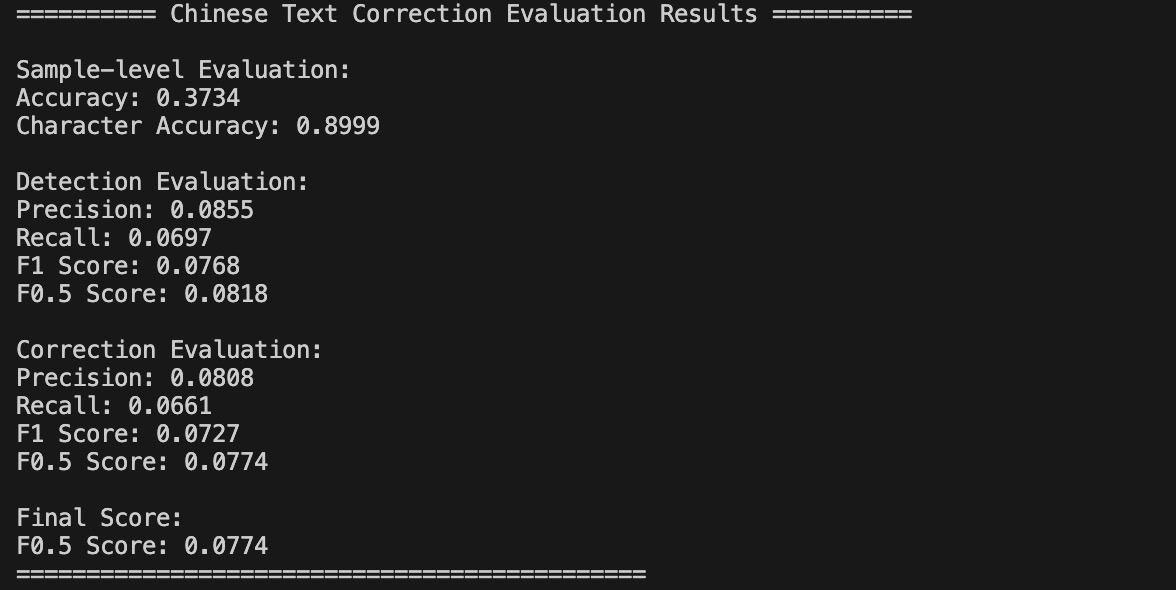
\includegraphics[width=1\textwidth]{../pic/rule.png} 
    \caption{rule}  
\end{figure}

说实话,rule这个方法是真的笨比,感觉不下降就很好了。

\subsubsection{方法2:ml模型}
这个板块分为ngram和ml方法,先看ngram吧:btw我稍微修改了一下类别的问题,单独把两个拆开了,变成了两个单独的类别,这样好修改\\
\medskip

\textbf{1.ngram模型}:\\
ngram模型主要是要修改\_train\_ngram\_model,对于这个东西,首先看他干了啥:很显然,现在是最简单的,一个gram的实现。
\begin{itemize}
    \item train部分:这个模块主要是对训练样本进行一元,二元,三元,四元的统计并更新counter。然后对错误label=1的进行分析,
    然后和目标文本对比,加入误差矩阵。并且储存每一个字的一个错误概率
    \item correct:主要是逐字去看错误概率,如果小于某个阈值就跳过。然后根据上下文纠错,看是否要纠正,然后用ngram进行选择。对比原字符看替换哪一个
\end{itemize}
那么对于这个,涉及到我到底看哪一个字符的评分,这个问题比较重要。事实上,好像把补全了之后没有很明显的提升,那就说明参数要调,还有一个问题是
除了参数,阈值这个东西在我看的里面确实做的不够。然后我更换了阈值和调参数,
具体操作:python3 main.py --method statistical --analyze 0 --statistical\_method ngram --statistical\_optparam 1.然后做出来的结果如下 \\
\begin{figure}[h]
    \centering
    \label{ngram}
    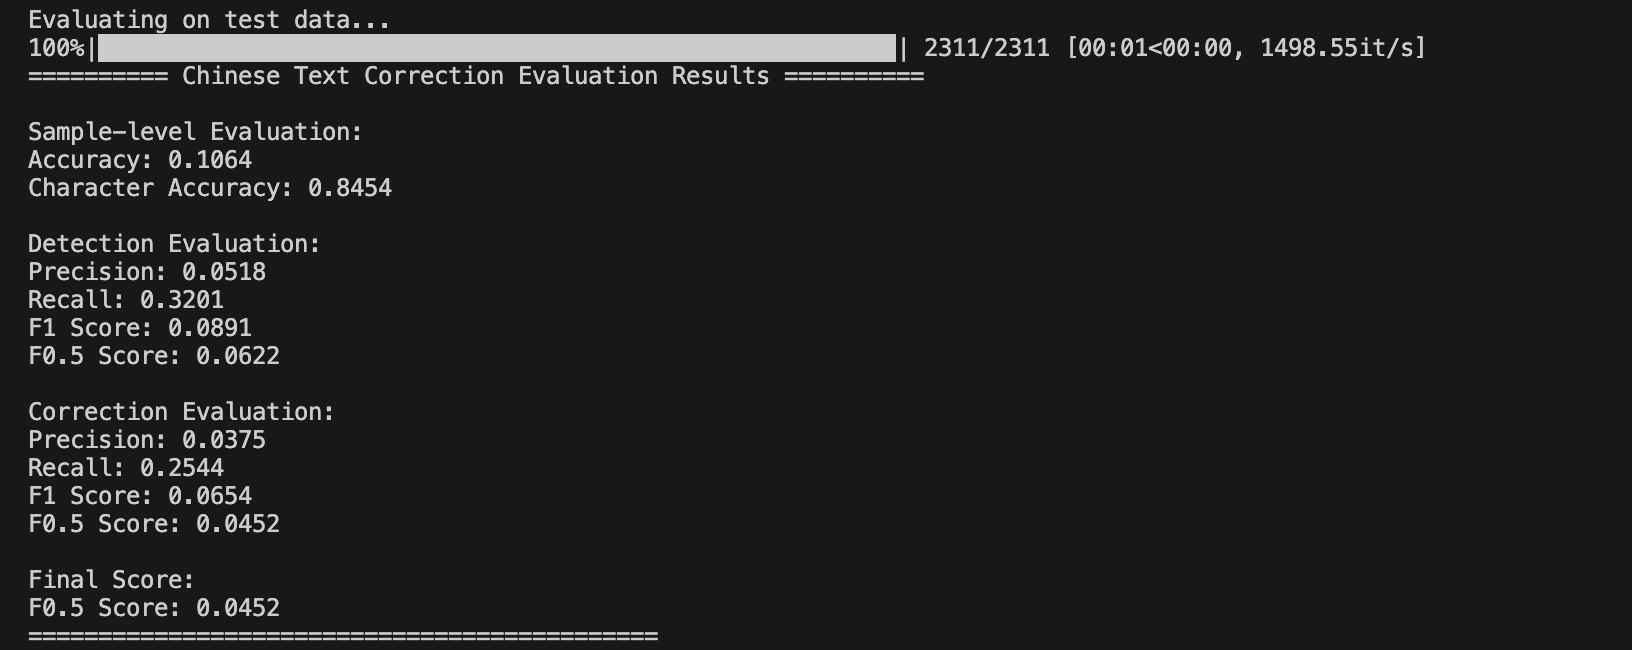
\includegraphics[width=1\textwidth]{../pic/ngram.png} 
    \caption{ngram}  
\end{figure}

从结果来看,这个任务用ngram的统计方法可能有点鸡肋了。

\medskip

\textbf{2.ml模型}:\\
1

\subsubsection{方法3:ensemble模型}

\subsection{其余方法}

\section{如何复现结果和代码环境依赖问题}

rulebase:
\textbf{复现指令:}
\begin{lstlisting}
    python3 main.py --method rule --analyze 0  
\end{lstlisting}

statistical ngram:
\textbf{复现指令:}
\begin{lstlisting}
    python3 main.py --method statistical --analyze 0 --statistical_method ngram 
    --statistical_optparam 0
\end{lstlisting}

statistical ml:
\textbf{复现指令:}
\begin{lstlisting}
    python3 main.py --method statistical --analyze 0 --statistical_method ml 
\end{lstlisting}



\section{不同实验方法的对比结果}

\section{一些简单思考}

\end{document}